%! Author = alessandromarcantoni
%! Date = 18/10/21

\section{Design architetturale}\label{sec:architectural-design}
Data la natura del progetto, si è ritenuto opportuno adottare astrazioni ben consolidate per quanto riguarda
l'architettura.

\subsection{Pattern Architetturali}
In particolare, dato che l'applicazione, in quanto gioco, prevede interazioni con l'utente si è deciso
di sfruttare il pattern \textbf{MVC}: uno dei più noti ed utilizzati.

L'adozione di tale architettura ci ha permesso di tracciare un'efficace separazione di responsabilità
tra i vari componenti:
ciò si è rivelato fondamentale, in fase di design e sviluppo del dominio, per concentrare la propria attenzione
sui propri task, senza quindi doversi preoccupare della rappresentazione.
Inoltre, un ulteriore vantaggio che questo pattern garantisce è quello di poter fornire una diversa
implementazione dell'interfaccia grafica senza dover applicare alcuna modifica ad altre porzioni dell'applicazione.

\subsection{Modello ad Attori}
La presenza di un elevato numero di entità all'interno dell'applicazione ha portato alla luce l'esigenza di gestire,
già a livello architetturale, la possibilità di sfruttare a pieno la potenza della cpu rendendo quindi il programma
concorrente. In particolare, per astrarre dalla gestione problematiche tipiche di sistemi concorrenti
(mutua eclusione e corse critiche) si è deciso di adottare un approccio basato su attori. Dal momento che ogni attore
incapsula al suo interno un flusso di controllo basato su \textit{event loop} e che le interazioni avvengono
esclusivamente attraverso scambio di messaggi, non è necessario gestire meccanismi di sincronizzazione.

Inoltre, abbiamo ritenuto il modello ad attori particolarmente adeguato per la realizzazione dell'applicazione
in quanto essi incapsulano un \textbf{comportamento}, il quale ben si adatta a descrivere l'effettivo comportamento
delle entità all'interno del modello. Tale scelta ci ha quindi garantito un livello di astrazione ed un'espressività
che ha positivamente influenzato anche le fasi successive di design ed implementazione.

\subsubsection{Vantaggi del Paradigma ad Attori}
Di seguito si elencano i vantaggi riscontrati a fronte dell'utilizzo del framework \textit{Akka}:
\begin{itemize}
    \item Espressività del codice relativo al comportamento delle entità di gioco.
    \item Migliore incapsulamento dei task di ogni componente.
    \item Maggior modularità del codice.
    \item Evitata la gestione della sincronizzazione mediante meccanismi quali semafori o monitor.
\end{itemize}

\subsection{Svantaggi del Paradigma ad Attori}
Nonostante l'effettiva potenza ed efficacia del paradigma, quest'ultimo comporta anche alcuni svantaggi:
\begin{itemize}
    \item Le uniche interazioni possibili tra componenti avvengono mediante scambio di messaggi.
    \item Possibilità di \textit{bottleneck} dovuta al message passing (in questo caso tale pericolo è ridotto in quanto il sistema sviluppato non è distribuito).
    \item All'aumentare delle dimensioni del sistema, il numero dei diversi messaggi che ogni attore deve gestire aumenta notevolmente.
\end{itemize}

\subsection{Architettura Complessiva}
Come conseguenza dell'adozione del modello ad attori, anche il pattern MVC adottato ha risentito dell'adozione di tale
paradigma. Di fatto, i componenti \texttt{Model}, \texttt{View} e \texttt{Controller} sono stati modellati come attori.
Ciascuno di essi gestisce messaggi di tipo diverso:
\begin{itemize}
    \item \texttt{Input} - è il tipo di messaggio accettato dal \texttt{Controller}. Questo genere di messaggi serve a mediare l'interazione tra \texttt{View} e \texttt{Model}; in particolare, comprende tutte le interazioni dell'utente con l'applicazione ma anche tutti gli aggiornamenti del \texttt{Model} per l'interfaccia grafica.
    \item \texttt{Render} - è il tipo di messaggio accettato dalla \texttt{View}. Dal momento che rappresentano un aggiornamento dell'interfaccia, questi messaggi sono esclusivamente inviati dal \texttt{Controller} o dal \texttt{GameLoop}.
    \item \texttt{Update} - è il tipo di messaggio accettato dal \texttt{Model}. Qualsiasi messaggio di \texttt{Update} rappresenta, per ogni attore del modello, una notifica di cambiamento all'interno del ciclo di aggiornamento del programma.
\end{itemize}
Nonostante la netta separazione dei task tra i principali componenti individuati, alcuni di questi risultavano
eccessivamente complessi, violando il \textit{Single Responsibility Principle}, pertanto, si è ritenuto opportuno
modularizzarli ulteriormente. Nello specifico, il componente più affetto da tale problema è stato il \texttt{Model};
infatti, senza un'adeguata suddivisione esso avrebbe dovuto comprendere diverse logiche (gestione delle entitá, delle
dinamiche di gioco, eccetera), accettando per ognuna di queste un elevato numero di messaggi. La soluzione è stata
quindi quella di introdurre un \textit{manager} per ogni logica, in modo che il \texttt{Model} effettui solo un
ridirezionamento dei messaggi, ricevuti da \texttt{Controller} e \texttt{GameLoop}, verso i \textit{manager} più
opportuni: tale pattern di delegazione è molto comune all'interno del paradigma ad attori e rende efficace la
suddivisione dei task all'interno del sistema.

\begin{figure}[H]
    \centering
    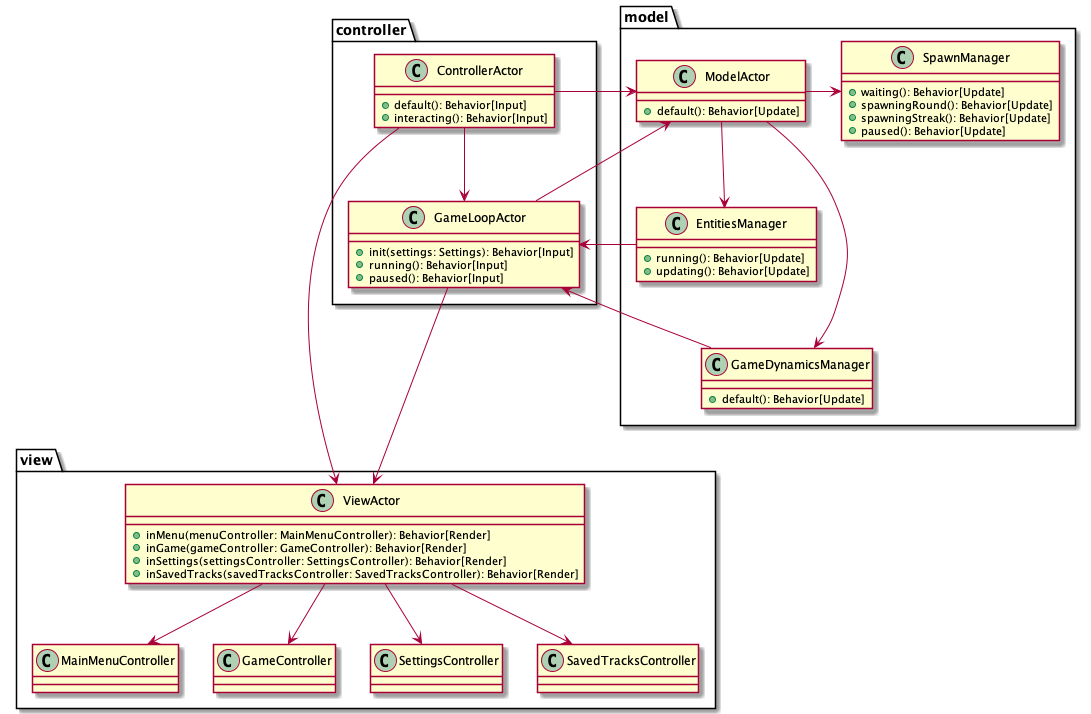
\includegraphics[width=\linewidth]{img/global-architecture}
    \caption{UML package diagram of the global MVC architecture.}
    \label{fig:global-architecture}
\end{figure}

La figura \ref{fig:global-architecture} mostra l'architettura appena descritta. Per modellare i principali attori del
sistema è stato utilizzato il formalismo UML; tuttavia, sono state adottate alcune convenzioni per facilitarne la
raffigurazione: in particolare, gli attori sono stati rappresentati come classi i cui metodi corrispondono ai loro
comportamenti. Tale scelta è stata motivata dall'effettiva implementazione degli attori che si rifà ad un pattern
consigliato da \textit{Akka}.
Inoltre, le relazioni tra package mostrate in figura potrebbero suggerire che il pattern MVC non venga pienamente
rispettato; tuttavia, queste ultime rappresentano in realtà il flusso dei messaggi. Infatti, i componenti del
\texttt{Model} non iniziano mai un'interazione verso il \texttt{Controller}, bensì si limitano a rispondere ai messaggi
di \texttt{Update}.
